\chapter{Implementation}
\label{ch:implementation}

Die Implementation der verschiedenen Deep-Learning Bilderkennungsmethoden erfolgte durch die Verwendung des Ultralytics YOLO \cite{Jocher_Ultralytics_YOLO_2023} Frameworks und der Eigenimplementation der U-Net \cite{ronneberger2015unetconvolutionalnetworksbiomedical} Architektur. Alle folgenden Modelle wurden auf einer NVIDIA GeForce RTX 3090 mit 24252 MiB Grafikkartenspeicher trainiert.

\section{Ultralytics YOLO}
Für die Extraktion von Diagrammen aus Texten, Schwierigkeitsklassifizierung von Liniendiagrammen und Instanzsegmentation der Wertelinien wurde das Ultralytics YOLO Framework verwendet. Es basiert auf der YOLO (You Only Look Once) Architektur, welche erstmal 2015 \cite{redmon2016lookonceunifiedrealtime} veröffentlicht wurde, und seit dem zehn Versionsiterationen durchlief. Unterstützt werden verschiedene Bild- und Videoerkennungsaufgaben, wie die Erkennung (detection), Segmentierung (segmentation), Posenschätzung (pose detection), Verfolgung (tracking) und Klassifizierung (classification). Das Ultralytics YOLO Framework ist anfängerfreundlich, die Verwendung erfolgt einfach, verfügt man bereits über einen annotierten Datensatz, kann mit lediglich einem Konsolenbefehl der Trainingsprozess des eigenen Modells gestartet werden. Ebenfalls verfügt es über der automatischen Datenagumentation während des Trainingsvorgangs und der Evaluation verschiedener Metriken des trainierenden und trainierten Modells.
\\
Ultralytics stellt zu dem Großteil der zehn YOLO Architekturen bereits vortrainierte herunterladbare Modelle bereit. Für das Vortrainieren der Objekterkennung, Klassifizierung und Instanzsegmentation wurde der COCO \cite{lin2015microsoftcococommonobjects} Datensatz verwendet, welcher aus über 200.000 Bildern besteht und  eingeteilt wurde auf 80 Objektklassen.

Diese werden außerdem in verschiedene Modellgrößen angeboten, sodass die Möglichkeit besteht zwischen Invarianzgeschwindigkeit, benötigte Gleitkommaoperationsleistungsfähigkeiten und verwendbaren Grafikkartenspeicher abwegegen zu können.
\\
Es wurden verschiedene YOLO Modelle verwendet, an denen jedoch keine Architekturänderungen vorgenommen wurden.
Sofern im Weiteren nicht explizit angegeben, wurden die Grundeinstellungen des Ultralytics YOLO Frameworks benutzt. Die genaue Anzahl der Trainingsepochen variierte zwischen den einzelnen Trainingsvorgängen, da bei allen die Geduldseinstellung (patience) von 100 Epochen verwendet wurde. Um die Überanpassung (over-fitting) an den Trainingsdatensatz zu vermeiden, wird mit diesem Geduldsparameter das Training vorzeitig abgebrochen, solange in den letzten beliebigen Epochen das trainierende Modell keine Verbesserungen der Validationsmetriken aufweisen konnte.

\subsection{Objekterkennung zur Extraktion von Diagrammen aus Texten}
\label{ch:objectdetection}

Für die Erkennung aller Diagrammen in den Vollseitscans wurde das YOLOv9e Modell verwendet.
\\
Zuerst wurde es auf den in \ref{ch:chartbank} beschreibenen, selbst erstellten DocBank Datensatz vortrainiert (pre-trained) und danach auf den Datensatz aus \ref{ch:scanbank}, der historischen Wirtschaftsscans, feintrainiert (fine-tuned). Beide Datensätze wurden mit der häufig verwendeten 80-20 Aufteilung differenziert. In diesem Fall werden 80\% des Datensatzes für das Trainieren und 20\% für das Evaluieren des Modells benutzt. Die hierbei 20\% des Evaluationssets bestehen aus Daten, welche das Modell vor dem Zeitpunkt noch nie gesehenen hat und dementsprechend unbekannt sind.
\\
Es wurde die Bildgröße von 1024x1024 Pixel verwendet und eine Batchgröße von 7 gewählt, da für eine höhere Batchgröße die verwendete Grafikkarte über ungenügend viel Speicher verfügte. Die von den Grundeinstellungen geänderten Parametern der Datenaugmentierung, mitsamt ihrer jeweiligen Wahrscheinlichkeiten, bestanden aus:

\begin{itemize}[itemsep=0pt, topsep=0pt]
    \item Farbmanipulation im HSV-Farbraum: Hue (1.0), Sättigung (1.0) und Helligkeit (0.5)
    \item BGR-Kanaländerung (0.5)
    \item Skalierung (1.0)
    \item Vertikales Spiegeln (0.1)
    \item Überlagern von Bildern (Mixup, 1.0)
\end{itemize}

Gewählt wurden diese Augmentierungstechniken mit dem Ziel die universelle Erkennungsfähigkeiten des trainierted Modells zu stärken. Farbmanipulationen helfen dem Modell zuversichtlichere Vorhersagen auf einer breiten Spanne unterschiedlicher Papierhintergründe zu treffen, beziehungsweise Diagramme mit willkürlichen Farben besser zu erkennen.

\clearpage


\subsection{Klassifizierung zur Schwierigkeitsbestimmung von Liniendiagrammen}

Der Trainingsvorgang der Schwierigkeitsklassifizierung der Liniendiagrammen folgte ähnlich der Objekterkennung aus \ref{ch:objectdetection}. Da hier das gewählte YOLOv8m-cls Modell nur Vorhersagen über bereits extrahierte Diagramme machen muss und nicht mehr über Vollseitscans, wurde die Bildgröße auf 640x640 Pixel reduziert. Im Vergleich zu der vorherigen Objekterkennung konnten keine Verbesserungen der Verwendung eines größeren Modells beobachtet werden, weshlab für die Klassifizierung lediglich das Modell mittlerer Größe gewählt wurde. Die Batchgröße dagegen wurde auf 16 erhöht und ebenfalls wurde wieder der Trainingsprozess durch den Geduldsparameter von 100 beendet, anstatt durch eine festgelegte Epochenbegrenzung. Die veränderten Augmentierungstechniken, sowie deren Parameter, bestanden aus:

\begin{itemize}[itemsep=0pt, topsep=0pt]
    \item Farbmanipulation im HSV-Farbraum: Hue (1.0), Sättigung (1.0) und Helligkeit (0.5)
    \item BGR-Kanaländerung (0.5)
    \item Vertikales Spiegeln (0.1)
    \item Rotation ($\pm$5°)
    \item Scherung ($\pm$5°)
    \item Zufälliges Löschen (1.0)
\end{itemize}

Auch wenn das Löschen zufälliger Bereiche im Bild möglicherweise kontraproduktiv wirkt, erziehlte die Verwendung dieser Technik zu besseren Ergebnissen, weshalb sie mit einbezogen wurde. Die restlichen Augmentierungen wurden für die breitere Diagrammsvarianz gewählt.

\begin{figure}[H]
    \centering
    \captionsetup{width=.75\linewidth}
    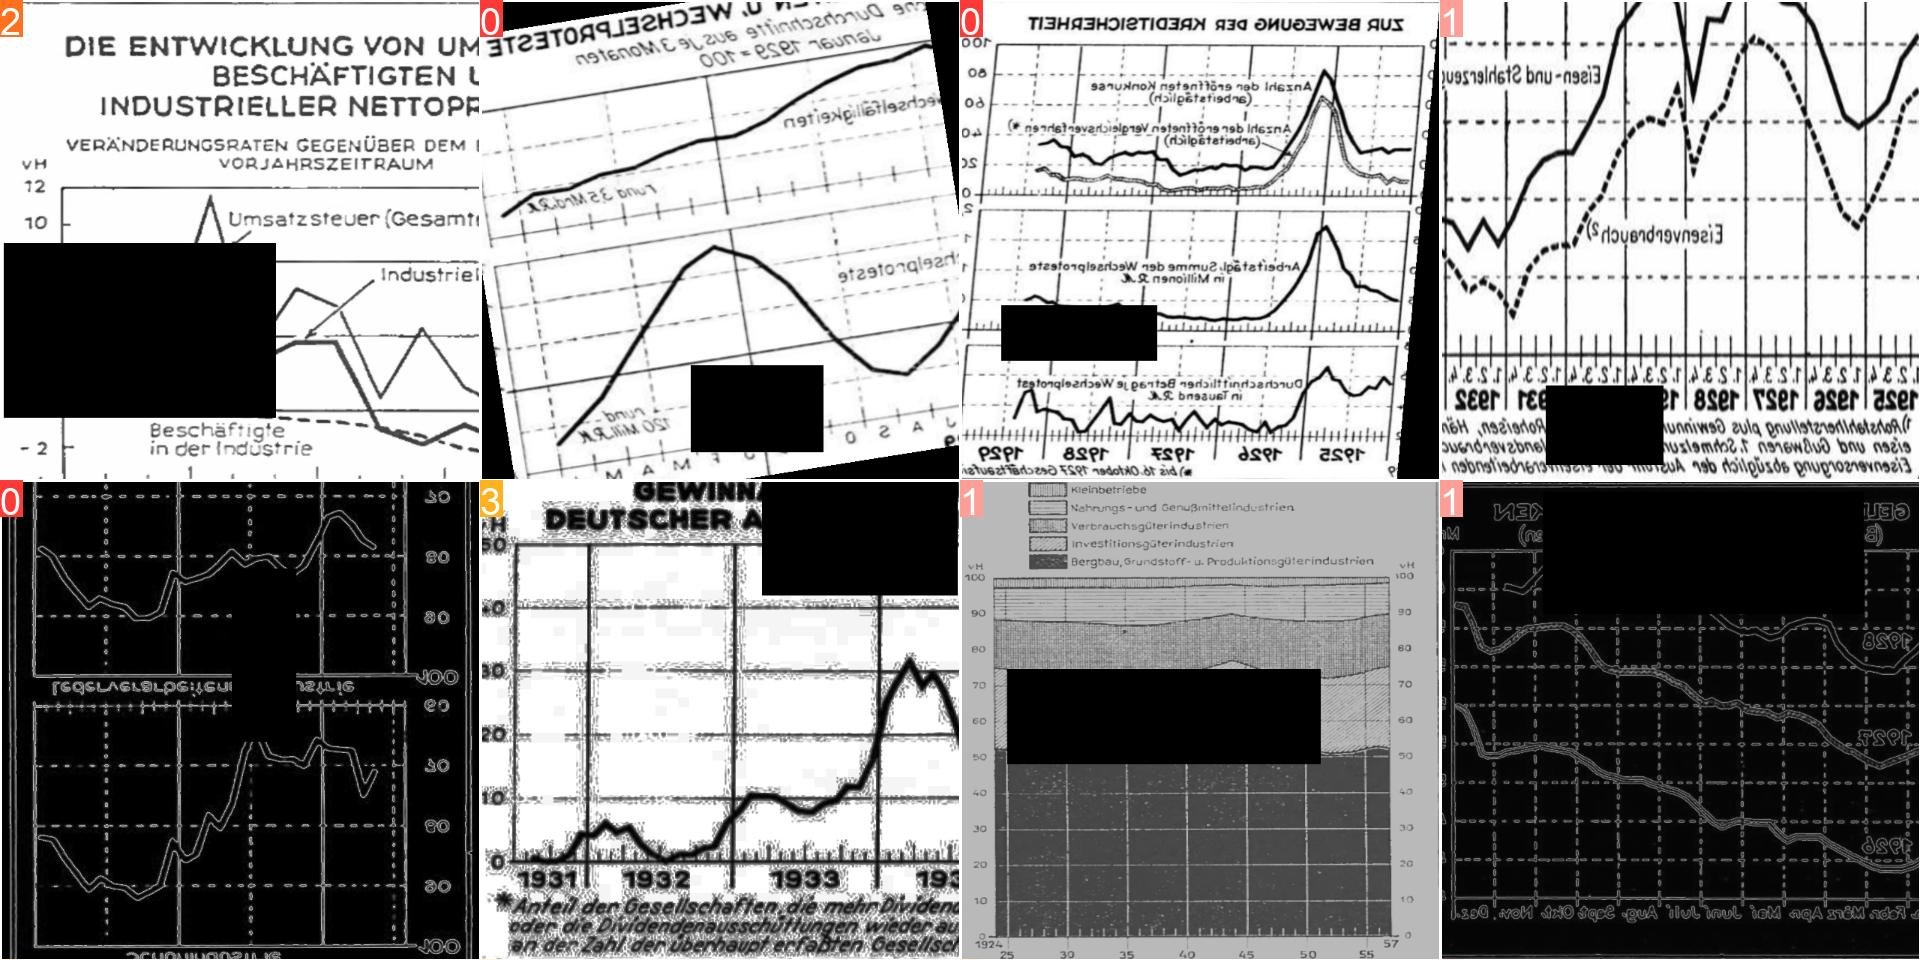
\includegraphics[width=.75\textwidth]{Implementation/img/classify_train_batch.jpg}
    \caption{\hbadness=10000 Augmentierter Trainingsbatch der Klassifizierung}
    \label{fig:classify_train_batch}
\end{figure}

Desweiteren wurde dieser beschriebene Trainingsprozess erneut auf der anderen Version, des in \ref{ch:linebank} beschriebenen, Datensatzes mit der Vereinigung der sich überlappenden und nicht überlappenden Wertelinien in die gemeinsame Klasse mehrerer Wertelinien trainiert.

\subsection{Instanzsegmentation von Wertelinien in Liniendiagrammen}

Die Instanzsegmentation durch Ultralytics YOLO erfolgte mithilfe der in \ref{ch:genlines} und \ref{ch:lines} definierten Datensätze der Wertelinien synthetischer und historischer Liniendiagramme. Wie zuvor beschrieben wurden diese zuerst in das, von dem Framework benötigte, Polygonannotationsformat konvertiert. Hierzu wurde Python in Verbindung mit der Bildverarbeitungsbibliothek OpenCV \cite{opencv_library} verwendet. Die Korrektheit der Konvertation von den Binärmasken in Polygonform wurde durch den von Ultralytics erstellten Trainingsbatches, als auch durch Auswertung mithilfe der Annotationswebseite Roboflow \cite{dwyer2024roboflow} überprüft werden. Im Anschluss konnte das YOLOv8x-seg Model mit einer Bildgröße von 512x512 Pixel und Batchgröße von 16 trainiert werden. Der Trainingsprozess verlief erneut in zwei Schritten.
Diese Parameter wurden für sowohl das Vortrainieren auf den synthetischen, als auch das Feintrainieren auf den  historischen Liniendiagrammen gewählt. Ebenfalls wurden für beie Trainingsprozesse dieselben Augmentierungstechniken verwendet:

\begin{itemize}[itemsep=0pt, topsep=0pt]
    \item Farbmanipulation im HSV-Farbraum: Hue (1.0), Sättigung (1.0) und Helligkeit (0.5)
    \item BGR-Kanaländerung (0.5)
    \item Vertikales Spiegeln (0.5)
    \item Rotation ($\pm$90°)
    \item Zufälliges Löschen (0.7)
    \item Überlagern von Bildern (Mixup, 0.5)
\end{itemize}

\begin{figure}[H]
    \centering
    \captionsetup{width=.75\linewidth}
    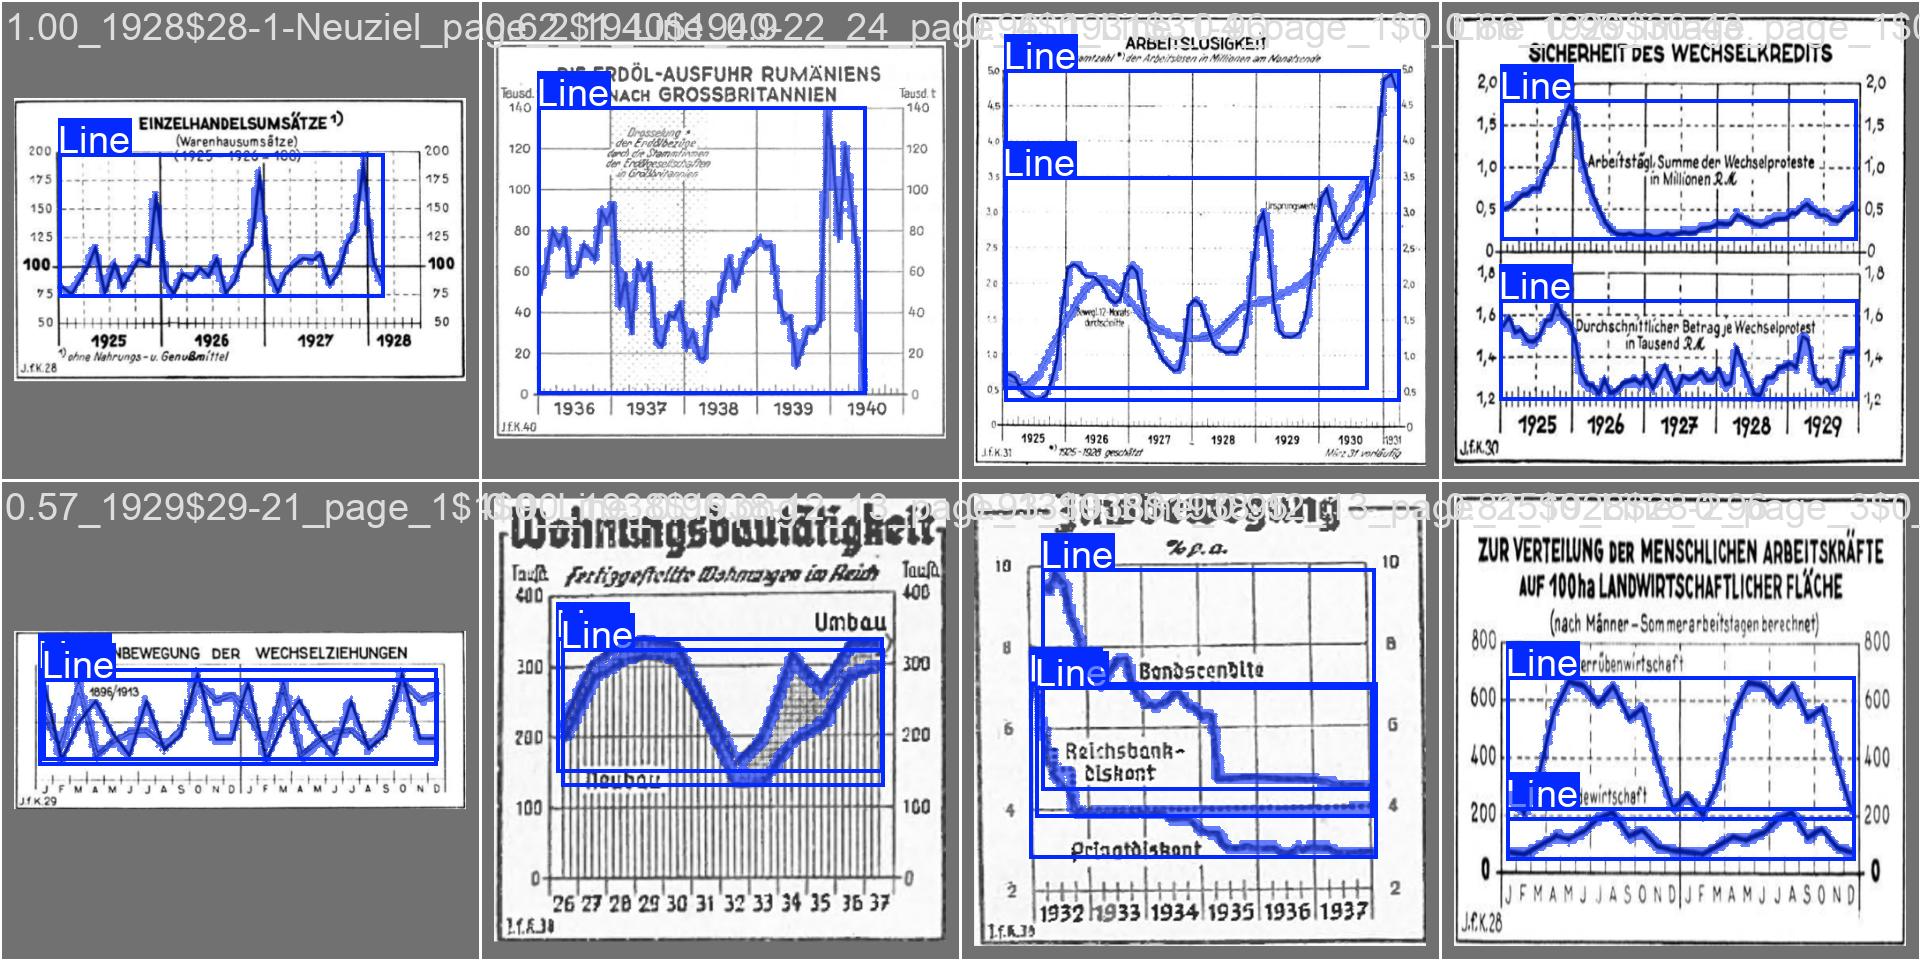
\includegraphics[width=.75\textwidth]{Implementation/img/instance_annotated.png}
    \caption{\hbadness=10000 Annotierte Wertelinien der Liniendiagrammen zur Instanzsegmentation}
    \label{fig:instance_annotated}
\end{figure}

Hier wurden stärkere Augmentierungstechniken gewählt, da Wertelinien unabhängig von Positionskontexten ausfindig gemacht werden müssen, weshlab additionell höhere Rotations- und Spiegelungsparameter verwendet wurden.


\section{U-Net: Semantische Segmentation von Wertelinien}

Als Alternative zur Instanzsegmentation wurde ebenfalls die semantische Segmentation durch die Eigenimplementation der U-Net Architektur verwirklicht. Diese wurde speziell für die medizinisch Bildsegmentierung und zeichnet sich besonders bei einer limitierten Anzahl von Trainingsdaten aus. Die Architektur des CNNs (convolutional neural network) kombiniert Encoder- und Decoderpfade mit Skip-Verbindungen um so präzise Segmentationsergebnisse zu erziehlen.
\\
Implementiert wurde die Datenvorverarbeitung, das Modelltraining und die Evaluation mithilfe der Keras API \cite{chollet2015keras}. Für die Augmentierung der Trainingsdaten wurde die Bibliothek Albumentations \cite{info11020125} genutzt. Lediglich der Code der U-Net Architektur selbst wurde in Form des Vanilla U-Nets \cite{zak2024kerasunet} übernommen.
\\
Der Ablauf des U-Net Trainings wurde wie folgt durchlaufen:
Zuerst wurde der Datensatz mithilfe verfügbarer Bibliotheksfunktionen eingelesen. Im Fall der Binärmasken wurde der Schwellenwert (threshold) von 30\% genutzt. Nach der Deklaration der Modellarchitektur wurde die Datenagumentation definiert. Folgende Augmentierungstechniken wurden verwendet:

\begin{itemize}[itemsep=0pt, topsep=0pt]
    \item Spiegeln entlang der horizontalen Achse (\texttt{A.HorizontalFlip}, \texttt{p=0.5})
    \item Spiegeln entlang der vertikalen Achse (\texttt{A.VerticalFlip}, \texttt{p=0.5})
    \item Drehung des Bildes (\texttt{A.RandomRotate90}, \texttt{p=0.5})
    \item Vertauschen von Breite und Höhe (\texttt{A.Transpose}, \texttt{p=0.5})
    \item Ausschneiden und Skalieren auf eine feste Größe (\texttt{A.RandomResizedCrop}, \texttt{height=512}, \texttt{width=512}, \texttt{scale=(0.8, 1.0)}, \texttt{p=0.5})
    \item Zuschneiden auf eine feste Größe vom Zentrum aus (\texttt{A.CenterCrop}, \texttt{height=512}, \texttt{width=512}, \texttt{p=0.5})
    \item Ausschneiden eines Bereichs des Bildes basierend auf der Maske (\texttt{A.CropNonEmptyMaskIfExists}, \texttt{height=512}, \texttt{width=512}, \texttt{p=0.5})
    \item Zufälliges Löschen von Bereichen (\texttt{A.CoarseDropout}, \texttt{max\_holes=8}, \texttt{max\_height=64}, \texttt{max\_width=64}, \texttt{p=0.5})
    \item Anpassung von Helligkeit und Kontrast (\texttt{A.RandomBrightnessContrast}, \texttt{p=0.5})
    \item Anwendung von Gamma-Korrektur (\texttt{A.RandomGamma}, \texttt{p=0.5})
    \item Zufälliges Mischen der Farbkanäle (\texttt{A.ChannelShuffle}, \texttt{p=0.5})
    \item Umkehren der Pixelwerte (\texttt{A.Solarize}, \texttt{threshold=128}, \texttt{p=0.1})
    \item Vollständiges Invertieren der Farbwerte (\texttt{A.InvertImg}, \texttt{p=0.1})
    \item Skalieren auf die maximale Größe entlang der längsten Kante (\texttt{A.LongestMaxSize}, \texttt{max\_size=512}, \texttt{p=1.0})
    \item Auffüllen auf eine Mindestgröße mit konstantem Rand (\texttt{A.PadIfNeeded}, \texttt{min\_height=512}, \texttt{min\_width=512}, \texttt{border\_mode=cv2.BORDER\_CONSTANT}, \texttt{value=0}, \texttt{p=1.0})
    \item Überlagern mit einem anderen Bild (\texttt{A.MixUp}, \texttt{p=1.0}, \texttt{alpha=0.7})
\end{itemize}

\section{Numerische Auswertung von Liniendiagrammen in Tabellenform}
abc



Für das Kapitel "Implementation" in Ihrer Bachelorarbeit über YOLO und U-Net sollten Sie sich auf die praktischen Aspekte der Umsetzung dieser Modelle konzentrieren. Hier sind einige Punkte, die Sie berücksichtigen sollten:

Technische Details der Implementierung:

Verwendete Programmiersprache und Frameworks (z.B. Python, PyTorch, TensorFlow)
Benötigte Hardware (GPUs, etc.)
Verwendete Bibliotheken und deren Versionen


Architektur-Anpassungen:

Spezifische Änderungen, die Sie an den Standard-YOLO- und U-Net-Architekturen vorgenommen haben
Begründung für diese Anpassungen


Datenaufbereitung:

Beschreibung der Datenvorverarbeitung
Augmentierungstechniken, falls verwendet


Hyperparameter:

Gewählte Hyperparameter (Lernrate, Batchgröße, etc.)
Begründung für die Wahl dieser Parameter


Training:

Kurze Beschreibung des Trainingsprozesses (Anzahl der Epochen, Optimierungsmethode)
Verwendete Loss-Funktionen


Inferenz:

Beschreibung, wie die trainierten Modelle für Vorhersagen eingesetzt werden


Herausforderungen und Lösungen:

Technische Schwierigkeiten, die während der Implementierung auftraten
Wie Sie diese Herausforderungen bewältigt haben



Die detaillierte Funktionsweise von YOLO und U-Net gehört eher in den theoretischen Teil oder in das Grundlagenkapitel Ihrer Arbeit. Die spezifischen Experimente, Ergebnisse und deren Auswertung sollten in einem separaten Kapitel "Experimente und Ergebnisse" behandelt werden.
Das Implementierungskapitel konzentriert sich auf die technischen Aspekte und praktischen Schritte, die Sie unternommen haben, um die Modelle für Ihr spezifisches Problem umzusetzen. Es bildet die Brücke zwischen der Theorie und den konkreten Experimenten.